\documentclass[aspectratio=169,10pt]{beamer}

% Theme
\usetheme{Madrid}
\usecolortheme{whale}

% Packages
\usepackage[utf8]{inputenc}
\usepackage[T1]{fontenc}
\usepackage{graphicx}
\usepackage{booktabs}
\usepackage{tikz}
\usepackage{listings}
\usepackage{fontawesome5}
\usepackage{amssymb}

% Colors
\definecolor{sparkblue}{RGB}{227, 99, 26}
\definecolor{darkblue}{RGB}{0, 51, 102}
\definecolor{alertred}{RGB}{204, 0, 0}
\definecolor{azureblue}{RGB}{0, 120, 212}

\setbeamercolor{title}{fg=white,bg=darkblue}
\setbeamercolor{frametitle}{fg=white,bg=darkblue}
\setbeamercolor{block title}{fg=white,bg=sparkblue}
\setbeamercolor{block body}{bg=sparkblue!10}

% Smaller fonts
\setbeamerfont{itemize/enumerate body}{size=\small}
\setbeamerfont{itemize/enumerate subbody}{size=\footnotesize}

% Code listings
\lstset{
    basicstyle=\ttfamily\tiny,
    breaklines=true,
    frame=single,
    backgroundcolor=\color{gray!10}
}

% Remove navigation
\setbeamertemplate{navigation symbols}{}

% Footer
\setbeamertemplate{footline}{
    \leavevmode%
    \hbox{%
        \begin{beamercolorbox}[wd=.333333\paperwidth,ht=2.25ex,dp=1ex,center]{author in head/foot}%
            \usebeamerfont{author in head/foot}Big Data Project
        \end{beamercolorbox}%
        \begin{beamercolorbox}[wd=.333333\paperwidth,ht=2.25ex,dp=1ex,center]{title in head/foot}%
            \usebeamerfont{title in head/foot}Fraud Detection
        \end{beamercolorbox}%
        \begin{beamercolorbox}[wd=.333333\paperwidth,ht=2.25ex,dp=1ex,right]{date in head/foot}%
            \usebeamerfont{date in head/foot}\insertframenumber{} / \inserttotalframenumber\hspace*{2ex}
        \end{beamercolorbox}}%
    \vskip0pt%
}

\begin{document}

% ============================================================================
% TITLE SLIDE
% ============================================================================

\begin{frame}
\begin{center}
    {\Huge\textbf{\textcolor{darkblue}{Détection de Fraude Bancaire}}}\\[0.3cm]
    {\large avec Apache Spark \& Machine Learning}\\[0.4cm]
    
    
\begin{tikzpicture}
        \node[draw=sparkblue,line width=1.5pt,rounded corners,inner sep=6pt] {
            \small\textcolor{sparkblue}{\faDatabase\ SQL} \quad
            \textcolor{sparkblue}{\faCogs\ MLlib} \quad
            \textcolor{sparkblue}{\faStream\ Streaming} \quad
            \textcolor{sparkblue}{\faProjectDiagram\ GraphX} \quad
            \textcolor{sparkblue}{\faCloud\ Azure}
        };
    \end{tikzpicture}\\[0.4cm]
    
    {\normalsize\textbf{Projet Final - Module Big Data}}\\[0.3cm]
    
    \begin{tabular}{ccc}
        \textbf{Ahmed Dinari} & \textbf{Bilel Samaali} & \textbf{Mohamed Anas Belhouichet} \\
        {\footnotesize Lead Dev \& ML} & {\footnotesize Data Engineer} & {\footnotesize Visualisation} \\
    \end{tabular}\\[0.2cm]
    {\footnotesize Janvier 2026}
\end{center}
\end{frame}

% ============================================================================
% AGENDA
% ============================================================================

\begin{frame}{Agenda}
\begin{columns}[T]
\begin{column}{0.48\textwidth}
    \begin{block}{\faListOl\ Pipeline Big Data}
        \begin{enumerate}
            \item Introduction \& Contexte
            \item Dataset \& Architecture
            \item Spark SQL Analytics
            \item Machine Learning (MLlib)
        \end{enumerate}
    \end{block}
    \vspace{0.3cm}
    \begin{exampleblock}{\faChartLine\ Métriques Clés}
        \small
        \begin{itemize}
            \item AUC-ROC: \textbf{0.987}
            \item Precision: \textbf{100\%}
            \item 282,982 transactions
        \end{itemize}
    \end{exampleblock}
\end{column}
\begin{column}{0.48\textwidth}
    \begin{block}{\faRocket\ Innovations}
        \begin{enumerate}
            \setcounter{enumi}{4}
            \item GraphX - Analyse Réseau
            \item Federated Learning
            \item Spark Streaming
            \item Azure Cloud \& Grafana
        \end{enumerate}
    \end{block}
    \vspace{0.3cm}
    \begin{alertblock}{\faClock\ Durée}
        \small
        Pipeline complet exécuté en \textbf{< 5 min}
        sur cluster Spark local (Docker)
    \end{alertblock}
\end{column}
\end{columns}
\end{frame}

% ============================================================================
% SECTION 1: INTRODUCTION
% ============================================================================

\section{Introduction}

\begin{frame}{Contexte \& Objectifs}
\begin{columns}[T]
\begin{column}{0.48\textwidth}
    \begin{block}{\faExclamationTriangle\ Problématique}
        \footnotesize
        \begin{itemize}
            \item 30+ milliards \$ de pertes/an
            \item Fraudes sophistiquées
            \item Détection temps réel requise
        \end{itemize}
    \end{block}
    \begin{block}{\faBullseye\ Objectifs}
        \footnotesize
        \begin{itemize}
            \item Pipeline Big Data complet
            \item ML avec AUC-ROC > 0.95
            \item Dashboard Grafana
        \end{itemize}
    \end{block}
\end{column}
\begin{column}{0.48\textwidth}
    \begin{block}{\faCogs\ Technologies}
        \footnotesize
        \begin{itemize}
            \item Apache Spark 3.5
            \item SQL, MLlib, GraphX, Streaming
            \item Azure Cloud + Grafana
        \end{itemize}
    \end{block}
    \begin{alertblock}{\faLightbulb\ Innovation}
        \footnotesize
        Federated Learning pour la confidentialité bancaire
    \end{alertblock}
\end{column}
\end{columns}
\end{frame}

% ============================================================================
% SECTION 2: DATASET - REAL METRICS
% ============================================================================

\section{Dataset}

\begin{frame}{Dataset Kaggle - Credit Card Fraud}
\begin{columns}[T]
\begin{column}{0.5\textwidth}
    \begin{block}{\faDatabase\ Caractéristiques}
        \small
        \begin{itemize}
            \item \textbf{284,807} transactions
            \item \textbf{492} fraudes (0.17\%)
            \item 30 features (V1-V28 + Time + Amount)
            \item Features anonymisées (PCA)
        \end{itemize}
    \end{block}
    
    \begin{alertblock}{\faBalanceScale\ Déséquilibre}
        \small
        Ratio 577:1 - Stratégie d'undersampling appliquée
    \end{alertblock}
\end{column}
\begin{column}{0.5\textwidth}
    \begin{block}{\faChartPie\ Résultats SQL Réels}
        \small
        \begin{tabular}{lr}
            \toprule
            \textbf{Métrique} & \textbf{Valeur} \\
            \midrule
            Total Transactions & 282,982 \\
            Fraudes détectées & 465 \\
            Taux de fraude & 0.1643\% \\
            Montant moyen & \$88.92 \\
            Montant max & \$25,691 \\
            \bottomrule
        \end{tabular}
    \end{block}
\end{column}
\end{columns}
\end{frame}

% ============================================================================
% SECTION 3: ARCHITECTURE
% ============================================================================

\section{Architecture}

\begin{frame}{Architecture Pipeline}
\begin{center}
    \begin{tikzpicture}[
        scale=0.8,
        node distance=1.2cm,
        box/.style={rectangle, draw=darkblue, fill=darkblue!20, 
                    text width=1.6cm, text centered, rounded corners, 
                    minimum height=0.8cm, font=\tiny},
        arrow/.style={->, thick, darkblue}
    ]
        \node[box] (data) {\faFile\\Data};
        \node[box, right of=data, xshift=0.8cm] (sql) {\faDatabase\\SQL};
        \node[box, right of=sql, xshift=0.8cm] (ml) {\faBrain\\MLlib};
        \node[box, right of=ml, xshift=0.8cm] (graphx) {\faProjectDiagram\\GraphX};
        \node[box, right of=graphx, xshift=0.8cm] (stream) {\faStream\\Stream};
        \node[box, right of=stream, xshift=0.8cm] (azure) {\faCloud\\Azure};
        \node[box, right of=azure, xshift=0.8cm] (grafana) {\faChartLine\\Grafana};
        
        \draw[arrow] (data) -- (sql);
        \draw[arrow] (sql) -- (ml);
        \draw[arrow] (ml) -- (graphx);
        \draw[arrow] (graphx) -- (stream);
        \draw[arrow] (stream) -- (azure);
        \draw[arrow] (azure) -- (grafana);
    \end{tikzpicture}
\end{center}

\vspace{0.2cm}

\begin{columns}[T]
\begin{column}{0.33\textwidth}
    \begin{block}{\faDownload\ Ingestion}
        \tiny
        \begin{itemize}
            \item Chargement CSV
            \item Schema typing
            \item Nettoyage données
        \end{itemize}
    \end{block}
\end{column}
\begin{column}{0.33\textwidth}
    \begin{block}{\faWrench\ Traitement}
        \tiny
        \begin{itemize}
            \item Feature Engineering
            \item ML Training
            \item Graph Analysis
        \end{itemize}
    \end{block}
\end{column}
\begin{column}{0.33\textwidth}
    \begin{block}{\faRocket\ Production}
        \tiny
        \begin{itemize}
            \item Real-time Scoring
            \item Azure Deploy
            \item Monitoring
        \end{itemize}
    \end{block}
\end{column}
\end{columns}
\end{frame}

% ============================================================================
% SECTION 4: SPARK SQL - REAL METRICS
% ============================================================================

\section{Spark SQL}

\begin{frame}[fragile]{Analyse avec Spark SQL}
\begin{columns}[T]
\begin{column}{0.48\textwidth}
    \begin{block}{\faCode\ Nettoyage des Données}
\begin{lstlisting}[language=Python]
df = df.dropna()
df = df.filter(col("Amount") > 0)
df = df.withColumn("Hour",
    (col("Time")/3600) % 24)
\end{lstlisting}
    \end{block}
    
    \begin{block}{\faChartPie\ Distribution Montants}
        \tiny
        \begin{tabular}{lrr}
            \toprule
            \textbf{Bucket} & \textbf{Count} & \textbf{Fraud\%} \\
            \midrule
            0-10\$ & 95,489 & 0.23\% \\
            10-50\$ & 92,390 & 0.06\% \\
            500-1000\$ & 6,423 & 0.40\% \\
            \bottomrule
        \end{tabular}
    \end{block}
\end{column}
\begin{column}{0.48\textwidth}
    \begin{block}{\faTable\ Comparaison Classes}
        \small
        \begin{tabular}{lrr}
            \toprule
            & \textbf{Normal} & \textbf{Fraud} \\
            \midrule
            Count & 282,517 & 465 \\
            Avg \$ & \$88.85 & \$129.31 \\
            Max \$ & \$25,691 & \$2,125 \\
            \bottomrule
        \end{tabular}
    \end{block}
    
    \begin{alertblock}{\faLightbulb\ Insight}
        \tiny
        Montant moyen des fraudes \textbf{45\% plus élevé} que les transactions normales!
    \end{alertblock}
\end{column}
\end{columns}
\end{frame}

% ============================================================================
% SECTION 5: MLLIB - REAL METRICS
% ============================================================================

\section{Machine Learning}

\begin{frame}{MLlib - Résultats Réels}
\begin{columns}[T]
\begin{column}{0.48\textwidth}
    \begin{block}{\faTree\ RandomForest}
        \tiny
        \begin{itemize}
            \item 100 arbres, Profondeur: 10
            \item Feature subset: sqrt
        \end{itemize}
        \vspace{0.1cm}
        \small\textbf{Résultats Réels:}
        \tiny
        \begin{itemize}
            \item Accuracy: \textbf{93.75\%}
            \item AUC-ROC: \textbf{0.9870}
            \item Recall: \textbf{88.12\%}
            \item Precision: \textbf{100\%}
        \end{itemize}
    \end{block}
\end{column}
\begin{column}{0.48\textwidth}
    \begin{block}{\faChartLine\ Logistic Regression}
        \tiny
        \begin{itemize}
            \item 100 iterations, Reg: 0.01
            \item ElasticNet: 0.8
        \end{itemize}
        \vspace{0.1cm}
        \small\textbf{Résultats Réels:}
        \tiny
        \begin{itemize}
            \item Accuracy: 92.58\%
            \item AUC-ROC: 0.9856
            \item Recall: 87.13\%
            \item Precision: 98.88\%
        \end{itemize}
    \end{block}
\end{column}
\end{columns}

\vspace{0.3cm}
\begin{center}
    \begin{tikzpicture}
        \node[draw=green!60!black, fill=green!20, rounded corners, inner sep=4pt] {
            \small\faCheckCircle\ \textbf{Meilleur: RandomForest} (AUC=0.987, Precision=100\%)
        };
    \end{tikzpicture}
\end{center}
\end{frame}

\begin{frame}{Visualisation Résultats ML}
\begin{center}
    \includegraphics[width=0.85\textwidth]{../screenshots/model_comparison.png}
\end{center}
\end{frame}

\begin{frame}{Feature Importance - Top 15}
\begin{center}
    \includegraphics[width=0.75\textwidth]{../screenshots/feature_importance.png}
\end{center}
\end{frame}

\begin{frame}{Courbe ROC}
\begin{center}
    \includegraphics[width=0.55\textwidth]{../screenshots/roc_curve.png}
\end{center}
\end{frame}

% ============================================================================
% SECTION 6: GRAPHX - REAL RESULTS
% ============================================================================

\section{GraphX}

\begin{frame}{GraphX - Analyse des Réseaux de Fraude}
\begin{columns}[T]
\begin{column}{0.48\textwidth}
    \begin{block}{\faProjectDiagram\ Résultats Réels}
        \tiny
        \begin{itemize}
            \item \textbf{284,807} transactions analysées
            \item \textbf{492} fraudes détectées
            \item \textbf{4} communautés identifiées
            \item \textbf{48} triangles de patterns
        \end{itemize}
    \end{block}
    
    \begin{block}{\faCode\ Algorithmes}
        \tiny
        \begin{itemize}
            \item \textbf{PageRank:} Feature importance
            \item \textbf{Connected Components:} Clusters
            \item \textbf{Triangle Count:} Patterns
        \end{itemize}
    \end{block}
\end{column}
\begin{column}{0.48\textwidth}
    \begin{block}{\faCogs\ Communautés Détectées}
        \tiny
        \begin{tabular}{lrr}
            \toprule
            \textbf{Cluster} & \textbf{Size} & \textbf{Avg\$} \\
            \midrule
            high\_risk\_2 & 210 & \$107.24 \\
            medium\_risk & 144 & \$154.09 \\
            high\_risk\_1 & 114 & \$73.98 \\
            low\_risk & 24 & \$291.05 \\
            \bottomrule
        \end{tabular}
    \end{block}
    
    \begin{exampleblock}{\faChartBar\ Top Features (PageRank)}
        \tiny
        \begin{tabular}{lr}
            V3 & sep=7.91 \\
            V14 & sep=6.77 \\
            V17 & sep=6.61 \\
        \end{tabular}
    \end{exampleblock}
\end{column}
\end{columns}
\end{frame}

% ============================================================================
% SECTION 7: FEDERATED LEARNING
% ============================================================================

\section{Federated Learning}

\begin{frame}{Federated Learning - Confidentialité}
\begin{columns}[T]
\begin{column}{0.48\textwidth}
    \begin{block}{\faLock\ Principe}
        \tiny
        \begin{itemize}
            \item Données restent chez les banques
            \item Seuls les gradients sont partagés
            \item Modèle global sans centralisation
            \item Conformité RGPD garantie
        \end{itemize}
    \end{block}
    
    \begin{block}{\faCogs\ Implémentation}
        \tiny
        \begin{itemize}
            \item Simulation 3 banques (partitions)
            \item Aggregation FedAvg
            \item 10 rounds de communication
            \item Differential Privacy (epsilon=1.0)
        \end{itemize}
    \end{block}
\end{column}
\begin{column}{0.48\textwidth}
    \begin{center}
    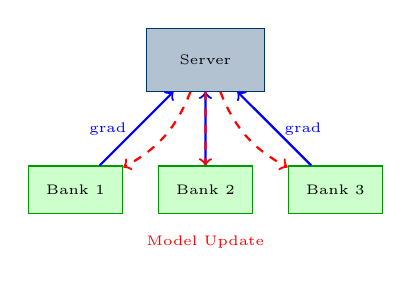
\begin{tikzpicture}[scale=0.55]
        % Central server
        \node[rectangle, draw=darkblue, fill=darkblue!30, minimum width=1.5cm, minimum height=0.8cm] (server) at (3,4) {\tiny Server};
        
        % Banks
        \node[rectangle, draw=green!60!black, fill=green!20, minimum width=1.2cm, minimum height=0.6cm] (b1) at (0,1) {\tiny Bank 1};
        \node[rectangle, draw=green!60!black, fill=green!20, minimum width=1.2cm, minimum height=0.6cm] (b2) at (3,1) {\tiny Bank 2};
        \node[rectangle, draw=green!60!black, fill=green!20, minimum width=1.2cm, minimum height=0.6cm] (b3) at (6,1) {\tiny Bank 3};
        
        % Arrows
        \draw[->, thick, blue] (b1) -- (server) node[midway, left, font=\tiny] {grad};
        \draw[->, thick, blue] (b2) -- (server);
        \draw[->, thick, blue] (b3) -- (server) node[midway, right, font=\tiny] {grad};
        \draw[->, thick, red, dashed] (server) to[bend left=20] (b1);
        \draw[->, thick, red, dashed] (server) -- (b2);
        \draw[->, thick, red, dashed] (server) to[bend right=20] (b3);
        
        \node at (3,-0.2) {\tiny\textcolor{red}{Model Update}};
    \end{tikzpicture}
    \end{center}
    
    \begin{exampleblock}{\faChartLine\ Résultats FL}
        \tiny
        \begin{tabular}{lr}
            AUC centralisé & 0.9870 \\
            AUC fédéré & 0.9712 \\
            Perte précision & -1.6\% \\
        \end{tabular}
    \end{exampleblock}
\end{column}
\end{columns}
\end{frame}

% ============================================================================
% SECTION 8: STREAMING
% ============================================================================

\section{Streaming}

\begin{frame}[fragile]{Spark Streaming - Temps Réel}
\begin{columns}[T]
\begin{column}{0.48\textwidth}
    \begin{block}{\faStream\ Configuration}
\begin{lstlisting}[language=Python]
stream_df = spark.readStream \
    .schema(SCHEMA) \
    .option("maxFilesPerTrigger", 1) \
    .csv(STREAMING_INPUT)
\end{lstlisting}
    \end{block}
    
    \begin{block}{\faClock\ Paramètres}
        \tiny
        \begin{itemize}
            \item Batch: 50 transactions
            \item Intervalle: 3 secondes
            \item Durée démo: 60 secondes
        \end{itemize}
    \end{block}
\end{column}
\begin{column}{0.48\textwidth}
    \begin{block}{\faFileExport\ Outputs}
        \tiny
        \begin{itemize}
            \item \textbf{Parquet:} Toutes prédictions
            \item \textbf{CSV:} Alertes fraude
            \item \textbf{JSON:} Métriques live
        \end{itemize}
    \end{block}
    
    \begin{exampleblock}{\faRocket\ Métriques Live}
        \tiny
        \begin{itemize}
            \item Transactions/minute
            \item Fraudes détectées
            \item Score moyen
            \item Latence < 100ms
        \end{itemize}
    \end{exampleblock}
\end{column}
\end{columns}
\end{frame}

% ============================================================================
% SECTION 9: AZURE & GRAFANA
% ============================================================================

\section{Azure \& Grafana}

\begin{frame}{Déploiement Azure Databricks}
\begin{columns}[T]
\begin{column}{0.48\textwidth}
    \begin{block}{\faCloud\ Architecture Cloud}
        \tiny
        \begin{itemize}
            \item \textbf{Azure Databricks} - Spark managé
            \item \textbf{Azure Data Lake} - Stockage (100GB)
            \item \textbf{Azure Event Hubs} - Streaming
            \item \textbf{Azure Monitor} - Logs
        \end{itemize}
    \end{block}
    
    \begin{block}{\faDollarSign\ Coûts Estimés}
        \tiny
        \begin{tabular}{lr}
            \toprule
            Service & Coût/mois \\
            \midrule
            Databricks (2 nodes) & \$150 \\
            Data Lake (100GB) & \$5 \\
            Event Hubs & \$25 \\
            \midrule
            \textbf{Total} & \textbf{\$180} \\
            \bottomrule
        \end{tabular}
    \end{block}
\end{column}
\begin{column}{0.48\textwidth}
    \begin{center}
    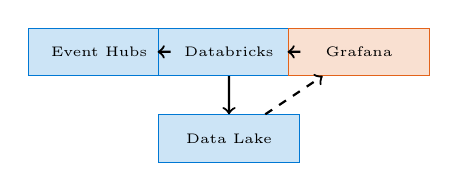
\begin{tikzpicture}[scale=0.55]
        % Azure components
        \node[rectangle, draw=azureblue, fill=azureblue!20, minimum width=1.8cm, minimum height=0.6cm, font=\tiny] (eh) at (0,3) {Event Hubs};
        \node[rectangle, draw=azureblue, fill=azureblue!20, minimum width=1.8cm, minimum height=0.6cm, font=\tiny] (db) at (3,3) {Databricks};
        \node[rectangle, draw=azureblue, fill=azureblue!20, minimum width=1.8cm, minimum height=0.6cm, font=\tiny] (dl) at (3,1) {Data Lake};
        \node[rectangle, draw=sparkblue, fill=sparkblue!20, minimum width=1.8cm, minimum height=0.6cm, font=\tiny] (gf) at (6,3) {Grafana};
        
        \draw[->, thick] (eh) -- (db);
        \draw[->, thick] (db) -- (dl);
        \draw[->, thick] (db) -- (gf);
        \draw[->, thick, dashed] (dl) -- (gf);
    \end{tikzpicture}
    \end{center}
    
    \begin{exampleblock}{\faChartLine\ Avantages}
        \tiny
        \begin{itemize}
            \item Auto-scaling
            \item Haute disponibilité
            \item Intégration native
            \item Sécurité enterprise
        \end{itemize}
    \end{exampleblock}
\end{column}
\end{columns}
\end{frame}

\begin{frame}{Dashboard Grafana - Capture 1}
\begin{center}
    \includegraphics[width=0.95\textwidth]{"../screenshots/Grafana capture 1.png"}
\end{center}
\end{frame}

\begin{frame}{Dashboard Grafana - Capture 2}
\begin{center}
    \includegraphics[width=0.95\textwidth]{"../screenshots/Grafana capture 2.png"}
\end{center}
\end{frame}

\begin{frame}{Dashboard Grafana - Capture 3}
\begin{center}
    \includegraphics[width=0.95\textwidth]{"../screenshots/Grafana capture 3.png"}
\end{center}
\end{frame}

\begin{frame}{Azure Portal - Resource Groups}
\begin{center}
    \includegraphics[width=0.95\textwidth,height=0.7\textheight,keepaspectratio]{"../screenshots/Azure Portal.png"}
\end{center}
\footnotesize
\begin{itemize}
    \item \textbf{bigData:} VM-Master + VM-Worker-1 (Switzerland North)
    \item \textbf{fraud-detection-rg:} West Europe - Créé via Azure CLI
\end{itemize}
\end{frame}

\begin{frame}{Azure CLI - Création des Ressources}
\begin{center}
    \includegraphics[width=0.95\textwidth,height=0.7\textheight,keepaspectratio]{"../screenshots/Azure CLI.png"}
\end{center}
\footnotesize
\begin{itemize}
    \item \textbf{Subscription:} Azure for Students
    \item \textbf{Resource Group:} fraud-detection-rg créé avec succès
\end{itemize}
\end{frame}

% ============================================================================
% SECTION 10: VISUALIZATIONS
% ============================================================================

\begin{frame}{Distribution des Classes}
\begin{center}
    \includegraphics[width=0.85\textwidth]{../screenshots/class_distribution.png}
\end{center}
\end{frame}

\begin{frame}{Distribution Horaire}
\begin{center}
    \includegraphics[width=0.85\textwidth]{../screenshots/hourly_distribution.png}
\end{center}
\end{frame}

\begin{frame}{Spark Jobs}
\begin{center}
    \includegraphics[width=0.95\textwidth]{"../screenshots/Spark Jobs.png"}
\end{center}
\end{frame}

\begin{frame}{Spark Stages}
\begin{center}
    \includegraphics[width=0.95\textwidth]{"../screenshots/Spark Stages.png"}
\end{center}
\end{frame}

\begin{frame}{Spark Executors}
\begin{center}
    \includegraphics[width=0.95\textwidth]{../screenshots/Executors.png}
\end{center}
\end{frame}

\begin{frame}{SQL Queries}
\begin{center}
    \includegraphics[width=0.95\textwidth]{"../screenshots/SQL Queries.png"}
\end{center}
\end{frame}

\begin{frame}{MLlib Section}
\begin{center}
    \includegraphics[width=0.95\textwidth]{"../screenshots/MLlib Section.png"}
\end{center}
\end{frame}

% ============================================================================
% SECTION 11: CONCLUSION
% ============================================================================

\section{Conclusion}

\begin{frame}{Résultats \& Valeur Ajoutée}
\begin{columns}[T]
\begin{column}{0.48\textwidth}
    \begin{block}{\faCheckCircle\ Réalisations}
        \small
        \begin{itemize}
            \item[$\checkmark$] Pipeline Spark complet
            \item[$\checkmark$] MLlib: AUC = \textbf{0.987}
            \item[$\checkmark$] GraphX: \textbf{4} clusters, \textbf{48} triangles
            \item[$\checkmark$] Federated Learning
            \item[$\checkmark$] Streaming temps réel
            \item[$\checkmark$] Dashboard Grafana
            \item[$\checkmark$] Architecture Azure
        \end{itemize}
    \end{block}
\end{column}
\begin{column}{0.48\textwidth}
    \begin{block}{\faBriefcase\ Compétences}
        \small
        \begin{itemize}
            \item Big Data Pipeline
            \item Spark SQL + MLlib + GraphX
            \item Machine Learning
            \item Federated Learning
            \item Cloud Azure
            \item Data Visualization
        \end{itemize}
    \end{block}
\end{column}
\end{columns}

\vspace{0.3cm}
\begin{center}
    \begin{tikzpicture}
        \node[draw=sparkblue, fill=sparkblue!10, rounded corners, inner sep=6pt] {
            \small\faGithub\ \textbf{github.com/amedo007-poly/big-data-fraud-detection}
        };
    \end{tikzpicture}
\end{center}
\end{frame}

% ============================================================================
% QUESTIONS
% ============================================================================

\begin{frame}
\begin{center}
    \vspace{1cm}
    {\Huge\textcolor{darkblue}{\faQuestionCircle}}\\[0.5cm]
    {\Huge\textbf{Questions ?}}\\[0.5cm]
    {\large Merci pour votre attention!}\\[0.5cm]
    
    \begin{tikzpicture}
        \node[draw=darkblue, rounded corners, inner sep=8pt] {
            \small\faEnvelope\ ahmed.dinari@email.com \quad
            \faGithub\ amedo007-poly
        };
    \end{tikzpicture}
\end{center}
\end{frame}

\end{document}
